\chapter{Audit du modèle : cohérence, validation, faiblesses}
\label{ch:audit}

Ce chapitre est un examen critique du modèle \emph{avant} toute conclusion. Il reprend les contrôles réalisés au cours
du projet (audit des mécanismes v0.5, contre-expertise v0.6) et les complète pour ce rapport. La règle suivie est de ne
masquer aucune faiblesse : lorsqu'une composante ne permet pas de conclusion quantitative fiable, cela est écrit.

\section{Cohérence dimensionnelle}

Toutes les équations de comportement portent sur des logarithmes ou des différences de logarithmes : elles sont
homogènes de degré zéro et sans dimension. Les termes de rappel comparent des grandeurs de même dimension (emploi et
production corrigée de la productivité ; consommation et revenu réel ; prix et coût unitaire). Les variables de niveau
sont exprimées en millions d'euros courants (revenus, recettes, dépenses, dette), en volumes aux prix de l'année de base
2022 (production, demande) ou en milliers de personnes (emploi, population). Trois points de vigilance ont été
vérifiés :
\begin{itemize}
\item le passage des volumes du tableau entrées-sorties (prix de base) aux volumes des comptes nationaux (prix
d'acquisition) se fait par des coefficients de conversion constants (\code{conv\_I} pour l'investissement) ;
\item les mesures exprimées en euros de 2025 sont indexées sur le PIB nominal de la référence, ce qui évite qu'une
mesure de 10\md{} perde la moitié de son poids relatif en vingt ans ;
\item \textbf{les volumes ne sont pas chaînés} (prix fixes de 2022) : sur vingt ans, la déformation des prix relatifs
(énergie, services) rend les agrégats en volume moins représentatifs. L'effet sur les écarts entre variantes est
faible ; il l'est moins sur les niveaux de très long terme.
\end{itemize}

\section{Cohérence comptable et conservation des flux}

\paragraph{Ce qui est garanti.} (1) Le cadre comptable M3 vérifie exactement, pour chaque année 2019-2025, que chaque
opération a autant d'emplois que de ressources et que la somme des capacités de financement des secteurs est nulle
\preuve{R}. (2) Le modèle de Leontief respecte l'équilibre ressources-emplois de chaque produit à chaque itération
(production + importations = consommations intermédiaires + demande finale). (3) La dette publique suit exactement
le solde public en projection.

\paragraph{Ce qui ne l'est pas.} Le modèle bouclé M8 n'est pas un modèle « stock-flux cohérent » complet :
\begin{itemize}
\item le revenu disponible des ménages est reconstruit par \emph{indexation} de ses composantes (salaires sur la masse
salariale, patrimoine sur le PIB nominal, prestations sur les prix) et non comme le solde d'un compte de ménages
alimenté par les paiements des autres secteurs ;
\item les comptes des sociétés et du reste du monde ne sont pas bouclés : rien n'oblige la somme des capacités de
financement des ménages, des entreprises, des administrations et du reste du monde à être nulle en projection ;
\item certaines recettes (« autres recettes ») et dépenses (« autres dépenses » : subventions, investissement public,
transferts divers) sont proportionnelles au PIB nominal. C'est une convention de référence : elle fait
\emph{augmenter} ces dépenses quand l'activité augmente, ce qui atténue l'effet favorable d'une mesure de croissance
sur le solde public, et l'inverse pour une mesure récessive.
\end{itemize}
La conséquence la plus visible est le \textbf{niveau du solde extérieur courant}, que le modèle situe à +2,9~\% du PIB
en 2025 alors que la Banque de France mesure un déficit de 11,6\md, soit $-$0,4~\% du PIB (chapitre~\ref{ch:reference}).
L'écart vient de revenus primaires nets reçus du reste du monde (3,1~\% du PIB en 2022 dans les comptes nationaux) qui
ne suivent pas leur évolution récente et d'échanges en volume aux prix de 2022. \textbf{Les niveaux de solde extérieur ne
sont donc pas utilisables ; seules les variations dues aux mesures le sont, avec prudence.}

\section{Doubles comptes et cohérence entre sous-modèles}

L'audit a recherché systématiquement les cas où un même effet serait compté deux fois. Deux erreurs ont été trouvées et
corrigées en version 0.6 \src{contre-expertise, section 8} :
\begin{enumerate}
\item \textbf{l'effet du coût d'usage du capital se cumulait chaque année} : l'effet de long terme d'une baisse d'IS ou
de taux était réappliqué à un investissement qui le contenait déjà, soit environ 3,5 fois l'élasticité estimée. La
baisse de l'IS de 25~\% à 20~\% augmentait l'investissement de 3~\% en 2035 au lieu de 0,9~\% ;
\item \textbf{l'investissement en logement était compté deux fois} dans les rétrosimulations (équation endogène et
indice exogène qui l'incluait).
\end{enumerate}
Pour ce rapport, trois autres risques ont été contrôlés :
\begin{itemize}
\item \emph{Microsimulation et équation de consommation} : la correction d'hétérogénéité (M14) n'utilise que le profil
\emph{relatif} des propensions ; la masse de revenu transférée n'est comptée qu'une fois dans le RDB. Contrôlé par
\code{tests/test\_m14\_identites.py}.
\item \emph{Mesures fiscales et recettes du modèle} : une hausse d'impôt est ajoutée aux recettes publiques et retirée
du revenu des ménages pour le même montant ; les pertes induites (moindre activité) passent par les assiettes du modèle,
pas par le chiffrage statique. Contrôlé sur chaque expérience (écart entre recette statique et amélioration du solde).
\item \emph{Additivité des mesures} : pour l'optimisation (partie~III), les effets de mesures simulées séparément sont
additionnés. Le test de validation montre que l'approximation additive est excellente pour les mesures budgétaires et
redistributives (écart de 0,01 point de PIB en 2032) mais \textbf{mauvaise pour les combinaisons de chocs d'offre et de
prix} : droits de douane + réindustrialisation + TVA + retour à 62 ans + énergie, PIB 2032 de $-$2,04~\% en simulation
complète contre $-$1,20~\% par addition \src{validation de l'additivité}. Tous les scénarios de la partie~III sont donc
re-simulés avec le modèle complet.
\end{itemize}

\paragraph{Cohérence des hypothèses entre sous-modèles.} Deux incohérences restent connues : (1) la microsimulation
fonctionne sur les revenus 2024 sans être revalorisée par les salaires et l'emploi simulés (couplage dans un seul sens,
micro vers macro) ; (2) les pensions de la référence sont calculées avec les prix et salaires de la référence, pas avec
ceux de chaque variante (un seul passage).

\section{Stabilité numérique}

La résolution annuelle converge en général en moins de 15 itérations avec un amortissement de 50~\%. Le module
européen ajoute quatre itérations externes. Les cas d'instabilité identifiés sont les combinaisons extrêmes de
paramètres dans la contre-expertise (dette s'écartant de plus de 25 points ou PIB de plus de 10~\%), écartées et
comptées. Aucune expérience de ce rapport n'a déclenché d'instabilité. Les résultats sont déterministes : relancer une
simulation donne les mêmes chiffres à $10^{-6}$ près.

\section{Ajustement historique}

\begin{figure}[htbp]
\centering
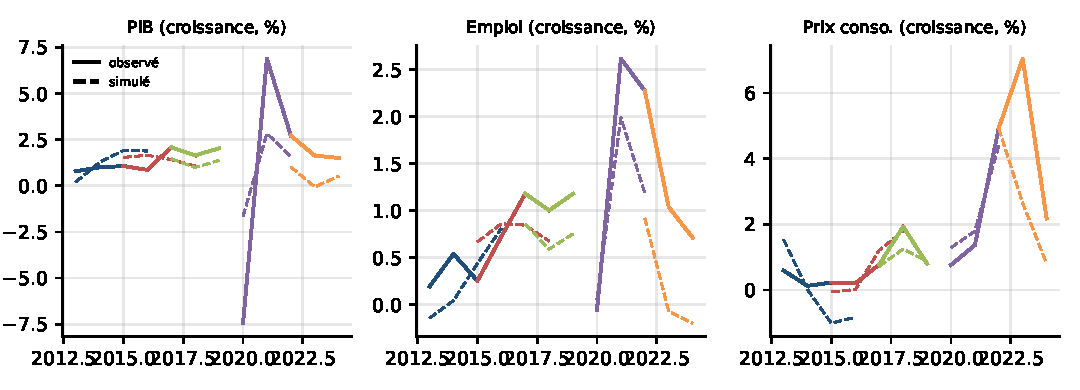
\includegraphics[width=\linewidth]{validation_retro.pdf}
\caption{Simulations hors échantillon : taux de croissance observés (traits pleins) et simulés (tirets), pour
plusieurs origines (estimation arrêtée à l'origine). Source : \code{outputs/validation\_hors\_echantillon.json}.}
\label{fig:validation}
\end{figure}

Le tableau~\ref{tab:retro} résume les tests rétrospectifs du modèle complet. En période calme (2015-2019), le modèle
reproduit la croissance, l'emploi, les prix et le solde public à moins de 1,5~\% ou 0,5 point près sur cinq ans. Il
prévoit mieux qu'un prolongement naïf l'investissement, les importations, l'emploi et les prix, \textbf{mais pas la
croissance du PIB} (erreur quadratique 0,64 point contre 0,50 pour la règle naïve sur 2015-2018). Il échoue sur
2022-2024 pour des raisons identifiées : la productivité a stagné (rétention de main-d'œuvre), les prix de l'énergie et
les marges ont suivi des dynamiques que le modèle ne représente pas.

\begin{table}[htbp]
\centering\small
\caption{Erreur de niveau du modèle complet en fin de période de rétrosimulation (simulé $-$ observé).}
\label{tab:retro}
\begin{tabular}{@{}lrr@{}}
\toprule
Variable & 2015-2019 (base 2014) & 2023-2024 (base 2022) \\
\midrule
PIB en volume & $-$1,0~\% (v0.6) & $-$3,5~\% \\
Investissement & $-$4,9~\% (v0.6) & $-$3,8~\% \\
Emploi & 0,0~\% & $-$0,6~\% \\
Prix à la consommation & +0,5~\% & $-$2,9~\% \\
Revenu disponible brut & +0,1~\% & $-$7,9~\% \\
Dette publique (points de PIB) & +0,4 & +2,0 \\
\bottomrule
\end{tabular}
\end{table}

\section{Sensibilité et robustesse}

La contre-expertise v0.6 a soumis le modèle à des sensibilités univariées sur 22 facteurs, à un criblage de Morris
(138 simulations par scénario) et à 50 tirages conjoints des coefficients estimés. Ses enseignements, qui conditionnent
la lecture de tout ce rapport, sont les suivants.
\begin{enumerate}
\item \textbf{Le facteur décisif n'est pas un coefficient estimé mais une hypothèse de bouclage} : la vitesse de la
fermeture d'offre $\rho$ (section~\ref{sec:fermeture}). Sa plage plausible (0 à 0,4) couvre une vision keynésienne
(la demande détermine durablement l'activité) et une vision classique (l'offre la détermine dès le moyen terme).
\item Les effets de court terme (1-2 ans) sont plus robustes que ceux de cinq ans et au-delà.
\item Le signe de l'effet d'une mesure sur le \textbf{solde public} est presque toujours robuste ; l'effet sur le
\textbf{ratio de dette} l'est beaucoup moins, car il dépend du niveau des prix (dénominateur), lui-même dépendant de la
courbe de Phillips et de l'indexation des salaires, deux paramètres mal identifiés.
\item Les réformes de l'âge de départ sont les mesures les plus incertaines : leur effet sur le PIB dépend de la manière
dont l'économie absorbe un supplément (ou une baisse) d'offre de travail.
\item Une dépense publique de 1 point de PIB a un multiplicateur de 1,26 la première année, 0,58 à cinq ans ; sans
fermeture d'offre 1,25 ; avec une fermeture forte, 0,13.
\end{enumerate}

\section{Ce que le modèle ne représente pas}
\label{sec:audit-manques}

\begin{limites}[Inventaire des faiblesses connues]
\begin{itemize}
\item \textbf{Bouclage de moyen terme non estimé} (fermeture d'offre) : premier facteur d'incertitude.
\item \textbf{Pas de bilans financiers} : pas d'effet de richesse, de patrimoine, de crédit ni de stabilité financière ;
une épargne placée à l'étranger ou en actifs existants n'est pas suivie.
\item \textbf{Pas d'anticipations} : pas d'effet de confiance, d'épargne de précaution liée aux déficits, ni d'effets
annoncés ; les écarts commencent en 2028.
\item \textbf{Emploi et salaires agrégés} : pas de distinction par qualification ; effet du SMIC et des allègements
ciblés mal représenté ; automatisation réduite à la substitution capital-travail.
\item \textbf{Dépenses publiques indistinctes} : santé, éducation, défense, recherche, fonctionnement ont le même effet ;
pas d'effet de l'éducation ou de la recherche sur la productivité ; seul l'investissement public améliore le potentiel.
\item \textbf{Énergie en valeur seulement} : pas de flux physiques, pas de substitution, pas d'émissions.
\item \textbf{Réindustrialisation exogène} : le modèle chiffre les conséquences d'un objectif de relocalisation, pas les
moyens de l'atteindre (aides, compétitivité, qualifications).
\item \textbf{Microsimulation statique, partielle en haut de distribution} : le dernier décile, et surtout le dernier
centile, sont mal représentés : une hausse de 10 points du taux de la tranche supérieure de l'IR rapporte
statiquement 1,7\md{} dans la microsimulation, montant probablement sous-estimé, puis 0,3\md{} seulement après les
réactions d'optimisation et de mobilité de M13 (de +1,0\md{} à $-$1,2\md{} selon l'élasticité retenue) ; les niveaux
de pauvreté et d'inégalités diffèrent de ceux de l'Insee.
\item \textbf{Retraites simplifiées} : pas de régimes, durée d'assurance, décote, réversion.
\item \textbf{Solde extérieur en niveau non fiable} ; RDB sous-estimé en 2023-2024.
\item \textbf{Dette à très long terme} : l'hypothèse d'un taux de 4,89~\% maintenu vingt ans sans réaction de
politique économique produit une dérive explosive de la référence (308~\% du PIB en 2047). Les niveaux de dette au-delà
de 2037 sont illustratifs ; seuls les \emph{écarts} entre scénarios sont interprétés, et avec prudence.
\end{itemize}
\end{limites}
